\documentclass[12pt]{article}


%%%%%%% PACKAGES (pode ser necessário acrescentar mais, dependendo do que se pretender inserir no documento) %%%%%%%
\usepackage[utf8]{inputenc}
 % para podermos escrever em português
\usepackage{geometry}
\newgeometry{left=2cm,bottom=2cm} 
\usepackage{setspace}
\onehalfspacing 


% para que o índice possa ter o título de ``Índice'' (caso contrário fica ``Conteúdo'')

\usepackage[nottoc,notlot,notlof]{tocbibind}

% para a inclusão de figuras
\usepackage{graphicx}

% para que não haja indentação no início dos parágrafos
\setlength{\parindent}{0pt} 

% para que os links apareçam como hiperligações
\usepackage{url}
\usepackage{hyperref}

\usepackage[usenames,dvipsnames]{color}    
%para introduzirmos fragmentos de script de R (ou de outra linguagem de programação)
\usepackage{listings} %para inserir excertos de codigo

\newcommand*{\authorimg}[1]{\raisebox{-.0\baselineskip}{\includegraphics[height=12pt,width=12pt,keepaspectratio,]{#1}}} %Para inserir o símbolo do R

\lstset{ 
  language=R,                     % linguagem
  basicstyle=\small\ttfamily, % tamanho das fontes usadas
  numbers=left,                   % onde colocar numeração das linhas de código
 numberstyle=\tiny\color{blue},  % estilo a usar para numeração das linhas
  stepnumber=1,                   % distância entre duas linhas numeradas (se for 1, cada linha será numerada)
  numbersep=5pt,                  % distância a que a numeração das linhas está do código
  backgroundcolor=\color{white},  % cor do background
  showspaces=false,               
  showstringspaces=false,         % sublinhar espaços em strings
  showtabs=false,                
  frame=single,                   % coloca uma moldura à volta do código
  rulecolor=\color{black},        % cor do frame
  tabsize=2,                    
  captionpos=b,                   % posição da legenda
  breaklines=true,                % line breaking automático
  breakatwhitespace=false,        
  keywordstyle=\color{RoyalBlue},      % estilo das keywords
  commentstyle=\color{YellowGreen},   % estilo dos comentários
  stringstyle=\color{ForestGreen}      % estilo das strings
} 
%%%%%%% INÍCIO DO DOCUMENTO %%%%%%%
\begin{document}
\thispagestyle{empty}
% CAPA
\begin{flushleft}

\includegraphics[scale=0.15]{ESTB.jpg}
\end{flushleft}

\begin{center}
\Large{Instituto Politécnico de Setúbal}
\end{center}

\begin{center}
\Large{Escola Superior de Tecnologia do Barreiro}
\end{center}

\medskip % para dar um espaço vertical


\begin{center}
\Large{\textbf{Laboratório em Bioinformática}}
\end{center}
\begin{center}
\Large{Licenciatura em Bioinformática}
\end{center}

\vspace{3cm} % espaço vertical (uma alternativa ao \medskip, que pode ser customizada para efeitos estéticos)

\begin{center}
\huge{\textbf{Automagic phylogenies}} 
\end{center}


\begin{center}
\Large{January, 2023}
\end{center}

\medskip
\begin{center}
\large{Group}

\large{Duarte Valente (202000053)}

\large{Gonçalo Alves (202000170)}

\large{Matilde Machado (202000174)}

\large{Rodrigo Pinto (202000177)}

\large{Guilherme Silva(202000178)}

\large{Marine Fournier(202000224)}
\end{center}

% FIM DA CAPA

\newpage
\pagenumbering{roman}
%\phantomsection

% Página com o índice
\tableofcontents

\newpage
\pagenumbering{arabic}

%%%%%%% SECÇÃO "INTRODUÇÃO" %%%%%%%
\section{Introduction}\label{sec:introducao} % a label pode ser o que se quiser
This report provides an overview of a software program designed to generate phylogenetic trees. Phylogenetic trees are graphical representations of evolutionary relationships among species or groups of organisms. The program utilizes various algorithms and data inputs to generate accurate and comprehensive phylogenetic trees. This report will provide a brief overview of the features and capabilities of the software, as well as its intended use and target audience. The software program is designed to be user-friendly and accessible for both researchers and educators in the field of evolutionary biology. It integrates advanced algorithms for tree construction, allowing for the analysis of large and complex datasets. The program also includes visualization tools for tree presentation, as well as options for customizing and annotating the tree output. Additionally, the software can import and export data in a variety of formats, making it easy to integrate with other analysis tools. The program is intended to provide a comprehensive and efficient solution for phylogenetic tree construction and analysis, and is an essential tool for anyone studying evolutionary relationships among species or groups of organisms.

\section{Background}\label{sec:desenvolvimentos}

In this section will be provided a quick background information on the field of phylogenetics and the challenges associated with creating phylogenetic trees.\newline
Phylogenetics is a study that aims to understand the evolutionary relationships among vast groups of similar organisms. It uses molecular biology to achieve to compare the genetic and morphological characteristics of different organisms, infering their evolutionary relationships. The main goal of this process is to construct evolutionary/phylogenetic trees, which depict the evolutionary relationships among different organisms.\newline
The process of creating a phylogenetic tree can be challenging. One of the main challenges is the availability of data. For example, it can be difficult to obtain high-quality genetic data for a certain group of organisms. The complexity of determining evolutionary relationships can be compounded by various factors such as, the method used, the type of data, and the assumptions made. Also, the construction of a phylogenetic tree assumes that similarities among organisms are the result of a shared ancestry, but it's possible that similarities may have developed independently within different groups of organisms.\newline
Finally, creating a phylogenetic tree requires making choices about the appropriate model and the appropriate method for inferring relationships, like Maximum likelihood, Bayesian and Distance-based methods. Selecting the most fitting model can be challenging, but fortunately, there are resources available to assist in making the best choice.\newline
The field of phylogenetics requires expertise from multiple areas, like molecular biology and computer science. Phylogenetic trees can offer significant insights into the evolutionary connections among organisms, however, it is crucial to keep in mind the difficulties and ambiguities that can arise during the creation of these trees.


\section{Methodology}\label{sec:desenvolvimentos}
The methodology for building phylogenetic trees involves several key steps, including data acquisition, data processing, and tree inference. Data acquisition involves obtaining high-quality genetic or morphological data for each of the organisms being analyzed. Data processing involves cleaning, organizing, and transforming the data into a format that is suitable for tree inference. Finally, tree inference involves using a variety of algorithms and models to construct the phylogenetic tree based on the processed data. In the next subsections it will be explained every part of the program from the data acquisition to the tree build and what methods were used.

\subsection{Environment and WorkFlow Management}
In order to ensure consistency and reproducibility of our program, we utilized Docker as our virtualization platform. Docker allowed us to package our software and dependencies into a single container, which could be run on any system with Docker installed. This eliminated the need for manual installation and configuration of dependencies, making our program easier to run and share.\newline
To manage and automate the execution of our program, we used Snakemake, a workflow management system. Snakemake enabled us to specify the dependencies and rules for our pipeline, making it easy to run and scale our program. The Snakemake file served as a blueprint for the pipeline, defining the input, output, and steps required to complete the program. This allowed us to simplify and streamline the execution process, while still maintaining full control and visibility over the workflow.\newpage

\subsection{Data Acquisition}
For the data acquisition we used the EntrezAPI, which The Entrez API is a component of the NCBI (National Center for Biotechnology Information) programmatic access to the vast collections of data maintained by the NCBI. The API provides a set of programmatic tools for accessing NCBI databases, including PubMed, GenBank, and others. The API allows developers to retrieve and manipulate data in a format that is suitable for analysis and integration into other programs or applications. The API supports a wide range of programming languages and platforms, making it a versatile and convenient tool for a wide range of scientific, medical, and research applications. The API is designed to be flexible, allowing developers to specify the data they need and the format they want it in, while also providing a variety of options for filtering, sorting, and transforming data to meet their specific needs. Overall, the Entrez API provides a powerful and flexible tool for accessing NCBI data and integrating it into a wide range of scientific and medical applications.\newline
The final output of the stage is a folder full of FASTA files that we will use to build the tree.
\subsection{Data processing}
As soon as the FASTA files were gathered, there are four necessary steps to make this FASTA files operable.\newline
The initial procedure involves assigning new, more descriptive labels to each sequence contained within each FASTA file, thereby rendering the information contained within each sequence more readily comprehended.\newline
The second step entails the alignment of each FASTA file, which will be executed utilizing the MAFFT software, which is a software tool for multiple sequence alignment. It can align large numbers of sequences efficiently and accurately, making it a popular choice in the field of molecular biology and genetics.\newline
The third operation involves the meticulous concatenation of all FASTA files, culminating in the creation of a comprehensive and unified file. To make this possible we used only python dictionaries. This procedure paves the way for conducting a maximum likelihood tree analysis, yet to undertake a Bayesian tree analysis, a final step is require.\newline
Finally, the final step involves tranforming the FASTA file into the NEXUS file format, with the aid of the SeqMagick tool, to optimize the data for further analysis, culminating in the creation of a Bayesian phylogenetic tree. SeqMagick is a powerful and flexible software package that allows for efficient manipulation and conversion of multiple sequence alignment (MSA) files in various formats.
\subsection{Tree Inference}
The end result of this phase will be the production of two distinct phylogenetic trees - one generated through the Maximum Likelihood method and the other, a Bayesian tree.\newline
To construct the maximum likelihood tree, it was imperative to utilize a FASTA file and the software of choice was RaxML. RaxML is a popular open-source software that uses maximum likelihood algorithms to construct phylogenetic trees from molecular sequence data. The implementation of RaxML within this project allowed for the efficient and accurate creation of the maximum likelihood tree.\newline
The final step in this phylogenetic tree building procedure will entail utilizing the NEXUS file and the MrBayes software to construct a Bayesian tree. A brief introduction to MrBayes, a widely-utilized software for Bayesian inference of phylogenetic trees, must also be provided to contextualize its application in this process.


\section{Implementation}\label{sec:desenvolvimentos}
The implementation phase is a crucial step in the development process where the methodology and techniques outlined in the previous stages are put into action. This phase involves executing the steps and methods that were designed and tested in the planning phase, resulting in the creation of a functional product or solution. The implementation phase, much like its predecessor, the methodology phase, will encompass four distinct stages of execution.
\subsection{Data acquisition}
To build the trees, the user was required to provide four arguments to the program, each of which helped to identify the specific combination of folders that were needed for the analysis. These arguments were crucial to ensuring that the correct data was used for each tree, and included the following:\newline
Scientific name of the species - This argument provided the scientific name of the species that was being analyzed, allowing the program to identify the relevant data and folders associated with that species.\newline
Taxonomy hierarchy - The taxonomy hierarchy argument was used to specify the hierarchical classification of the species being analyzed, allowing the program to determine the correct data and folders to use in the analysis.\newpage
Proximity - The proximity argument indicated the proximity between the sequences being analyzed, it would indicate how closely related two organisms are, the higher the percentage, higher the relationship between organisms.\newline
Similarity - The similarity argument indicated the level of similarity between the sequences being analyzed, is a measure of how alike two or more sequences or organisms are, based on their genetic or physical characteristics. The higher the similarity value, the more similar these two organisms are.\newline
To obtain the specific taxonomy rank, the user was required to provide two key inputs - the name of the species and the desired taxonomy hierarchy. The taxonomy rank refers to the hierarchical classification of organisms within a taxonomic system, and is used to provide insight into the evolutionary relationships between different species.\newline
For example, if the user entered "homo sapiens" as the name of the species and "order" as the desired taxonomy hierarchy, the program would conduct a search for all primates. By restricting the search based on proximity and similarity, the program was able to identify the specific FASTA folder that was needed for the analysis.\newline
To perform this search, the ENTREZ API was used, which provides direct access to the NCBI database. This database contains a wealth of information on the taxonomy and evolution of different species, and is an indispensable tool for researchers in fields such as biology, genetics, and ecology. By utilizing the ENTREZ API, the user was able to streamline the process of identifying the correct data and folders needed for the analysis, saving time and effort and allowing them to focus on the more complex aspects of their research.
\subsection{Data Processing}
\subsubsection{Fasta Handling}
After getting the FASTA folder, it was necessary to change the names of each sequence in each FASTA file inside the folder. The list of names was obtained from the FiltredScientificNames\_list.txt (an output from the data acquisition phase) and using the SeqIO module, a new folder containing FASTA files was generated, with each file named according to the corresponding sequence. An example of a sequence name, which initially appeared as "\>KC836121.1 Montifringilla ruficollis mitochondrion, complete genome," was transformed to "Montifringilla ruficollis" after processing with the SeqIO module.
\subsubsection{Fasta Alignment}
The alignment of the FASTA files was accomplished by converting the folder containing the FASTA files into a list, and then using a for loop to iterate through the list and align each FASTA file with the MAFFT command. Tshe aligned FASTA files were stored in a separate folder for easy access and organization. An example of an alignment FASTA can be seen in figure \ref{fig:aliview}
\subsubsection{Fasta Concatenation}
The process of concatenating the FASTA files involved reading each file in the folder of aligned FASTA files, line by line. For each file, the names of the sequences were extracted and used as the keys in a dictionary. The sequences themselves were assigned as the values for each key, providing a clear and structured representation of the data.
By using a dictionary to store the sequences, it was possible to easily access and manipulate the data, making further analysis and processing more efficient. The concatenated FASTA file provided a comprehensive and organized representation of all the sequences, ready for further analysis and interpretation. The concatenated FASTA will also be used to build both trees.
\subsection{Tree Inference}
\subsubsection{Maximum Likelihood Tree}
Prior to constructing a maximum likelihood tree, it is crucial to determine the most appropriate evolutionary model of DNA or protein sequence evolution. This can be achieved through the use of software tools such as modeltest-ng, which performs model selection and averaging in phylogenetic analysis. modeltest-ng compares multiple models of molecular evolution and calculates the likelihood of each model, based on the Akaike information criterion (AIC) or Bayesian information criterion (BIC). In this particular case, it was necessary to determine if the selected evolutionary model included the "+I" derivation. After knowing if the model included the "+I" derivation,The time had come to construct the tree using the RaxML command line tool. This command was designed to automatically execute a specified number of times using the "-\# autoFC" option, with the goal of generating a newick format file. This file, which serves as the output of the RaxML analysis, will then be utilized to visualize the tree and provide valuable insights into the evolutionary relationships between the sequences in the dataset. By executing the RaxML command in this manner, the user was able to perform a robust and efficient analysis to gain a better understanding of the evolutionary history of the sequences.
\subsubsection{Bayesian Tree}
The construction of the Bayesian tree posed a slightly different challenge than other types of phylogenetic trees. To begin the process, it was necessary to convert the concatenated FASTA file into a NEXUS file, which is a format that MrBayes, a popular Bayesian phylogenetic analysis software, can work with. This conversion was accomplished using SeqMagick, a powerful Python library designed specifically for the manipulation of biological sequences and sequence files.\newline
Once the necessary inputs had been prepared, the final step was to incorporate the MrBayes command lines into the NEXUS file. This step was crucial, as it ensured that all necessary commands would be executed automatically when MrBayes was run. This streamlined the analysis process and reduced the burden of manual intervention, freeing the user to focus on the interpretation and analysis of the results.\newline
By combining the powerful capabilities of SeqMagick and MrBayes, the user was able to efficiently and effectively build a Bayesian tree, gaining valuable insights into the evolutionary relationships between the sequences in the dataset. This type of analysis is critical for understanding the underlying mechanisms driving evolutionary change, and is a critical tool for researchers in many fields, including biology, genetics, and ecology.
\subsection{Test Suite}
To ensure the accuracy of our results, a comprehensive test suite was implemented throughout the phylogenetic tree building process. The test suite consisted of a series of validation checks for each step, starting the data acquisition with EntrezAPI, to the final phylogenetic tree output using MrBayes. The validation checks included verifying the integrity of input data, examining the alignment quality, and evaluating the consistency of tree topology. The results of the tests were recorded and analyzed to ensure that the program meets the required standards and produces accurate phylogenetic trees. The test were implement using pytest. Pytest is a popular testing framework for Python programming language that is used to write and run tests for applications and libraries. It allows developers to write tests in a simple, concise and readable manner. Pytest provides a rich set of tools for writing tests, including fixtures for setup and teardown, assertion introspection and plugins for extended functionality.

\section{Results}\label{sec:desenvolvimentos}
When embarking upon the examination of a phylogenetic tree, there are some important points that must be considered and valued. To evaluate the reliability and accuracy of the tree generated by our program, it is important to compare it with a tree derived from a prior study that has evaluated the same set of organisms.

After some discussion on the subject, it was deemed fitting to proceed with the analysis of the phylogeny of the Short-beaked Common Dolphin (Delphinus delphis) due to the moderate length of its genetic spectrum. With the program's implementation, we were able to successfully derive the phylogenetic tree of Delphinus delphis, utilizing the taxonomic rank of family and incorporating both percentage of similarity and proximity, with a value of 30.

Due to some research work, we were able to find an article that evaluates the phylogeny of our common dolphin Delphinus delphis. The article "Characterization of the complete mitochondrial genome and phylogeneticanalysis of the common dolphinDelphinus delphis(Cetacea: Delphinidae)" was written by Kyunglee Lee, JunMo Lee, Yuna Cho, Hawsun Sohn, Young-Min Choi, Se Ra Lim, Hye Kwon Kim,Sun-Woo Yoon, Dae Gwin Jeong and Ji Hyung Kim, who are mainly researchers from the National Institute of Fisheries Science, Republic of Korea and Korea Research Institute of Bioscience \& Bio Technology, Republic of Korea. This article evaluates the complete mitogenome of the common dolphin, Delphinus delphis. The overall structure of the 16,387 bp mitogenome was found to be very similar to those of other delphinid species, including ancient D. delphis individuals. A multigene phylogeny revealed that D. delphis was most closely related to Stenella coeruleoalba, and clustered well with other species within the subfamily Delphininae.

Upon scrutinizing both trees (Our tree can be seen in figure \ref{fig:ourPhy} and the article tree can be seen in figure \ref{fig:theirPhy}) it can be observed that there are several similarities between both trees, signifying that our program was able to obtain results that are, at the very least, promising. The article tree contains several organisms that we were unable to find in our trees, as the analysis performed by the researchers covers more distant mitochondrial genes of the Delphinus Delphis family organisms. Howeverthere are many other organisms that are common to both trees, such as those belonging to the Delphinidae family, which are represented by a clade in figuere \ref{fig:theirPhy}. Upon evaluating this clade, we can see that only a few organisms are not represented in the tree generated by our program figure \ref{fig:ourPhy}, such as Lagenorhynchus obliquidens, Lagenorhynchus albirostris and Lagenodelphis hosei. This clade is composed and diverges into 6 nodes leading up to our target organism, Delphinus Delphis. In comparison, our tree displays 8 nodes \ref{fig:ourPhy}, indicating the incorporation of more organisms. An attempt to further understand this difference reveals that the genus Sousa and Stenella feature more species in our tree than in the article tree, specifically Sousa Teuszii, Stenella longirostris, Stenella Frontalis and Stenella Clymene.\newline
It is also worth mentioning that several discrepancies can be seen in evolutionary terms, such as the fact that in the article tree \ref{fig:theirPhy}, the genus Sousa did not emerge as the ancestor of the entire Delphinidae family, as our tree \ref{fig:ourPhy} had suggested. Instead, it was the genus Stenella that diversified and later gave rise to Delphinus Delphis.\newline
Turning our attention to the other clade that can be identified, we can see many more differences between the different organisms in the two trees, despite the fact that almost all of the species are common to both. An interesting point to note is that the genus Lagenorhynchus, comprised of 3 species, was not represented in the article tree \ref{fig:theirPhy}, but was present in our program's tree \ref{fig:ourPhy}. This further underscores the comprehensive nature of our tree \ref{fig:ourPhy}, as it encompasses a wider range of species in general.\newline
On the same clade, we can see that the genus that originated all the others was Cephalorhynchus, and the one that appeared more recently was Globicephala, which can be seen in both trees. Generally speaking, the two trees are strongly identical. \newline
From the ancestor to Globicephala, we can then observe 7 nodes in the article's tree \ref{fig:theirPhy}, which is not much different from the program tree \ref{fig:ourPhy} which shows 10 nodes.\newline
To conclude, we can see some differences between the two trees at the level of the genus and species presented, which can be justified by the similarity and proximity percentage defined in the begining as parameters, but generally speaking, the two trees are very similar, which ends up being gratifying for our program because it indicates that the trees generated by our program are close to reality, confirming the reliability of them.
\newpage

%%%%%%% SECÇÃO "CONCLUSÕES" %%%%%%%
\section{Conclusion}\label{sec:conclusoes}
In conclusion, this program is a valuable tool for constructing both maximum likelihood and Bayesian trees, providing a comprehensive view of evolutionary relationships between different species. The implementation of these two methods allows for a comparison between two commonly used approaches in evolutionary biology. Maximum likelihood trees are based on the optimization of likelihood scores, whereas Bayesian trees incorporate prior knowledge and use a probabilistic framework to infer evolutionary relationships. However, the configuration of the Docker part of the program was a challenge for the team as it was their first time using it. Additionally, the integration of the ENTREZ API proved to be the most difficult aspect of the project, requiring significant effort to ensure its proper functioning. With the use of this program, researchers will be able to make informed decisions and choose the most appropriate tree-building method for their specific data and research questions.

%%% Bibliografia
\newpage
\begin{thebibliography}{}

\bibitem{Entrez}
\href{https://www.ncbi.nlm.nih.gov/books/NBK25501/}{Entrez API, Bethesda (MD): National Center for Biotechnology Information (US); 2010-.}

\bibitem{mafft}
\href{https://mafft.cbrc.jp/alignment/software/}{man2html, Time: 02:26:04 GMT, August 14, 2007}

\bibitem{seqmagick}
\href{https://seqmagick.readthedocs.io/en/0.4.0/}{SeqMagick documentation. (n.d.). SeqMagick. }
\bibitem{docker}
\href{https://docs.docker.com}{Docker, Inc. (2021). Docker. }

\bibitem{modeltest}
\href{https://github.com/ddarriba/modeltest}{Darriba, D., Posada, D., Kozlov, A. M., Stamatakis, A., Morel, B., \& Flouri, T. (2020). ModelTest-NG: a new and scalable tool for the selection of DNA and protein evolutionary models. Molecular Biology and Evolution, 37(1), 291-294.}
 
\bibitem{snakemake}
\href{https://f1000research.com/articles/10-33/v1}{Mölder, F., Jablonski, K.P., Letcher, B., Hall, M.B., Tomkins-Tinch, C.H., Sochat, V., Forster, J., Lee, S., Twardziok, S.O., Kanitz, A., Wilm, A., Holtgrewe, M., Rahmann, S., Nahnsen, S., Köster, J., 2021. Sustainable data analysis with Snakemake. F1000Res 10, 33.}

\bibitem{article}
\href{https://www.tandfonline.com/doi/epdf/10.1080/23802359.2018.1473720?needAccess=true&role=button}{Kyunglee Lee, JunMo Lee, Yuna Cho, Hawsun Sohn, Young-Min Choi, Se Ra Limc, Hye Kwon Kim, Sun-Woo Yoon, Dae Gwin Jeong, Ji Hyung Kim. (2018). Characterization of the complete mitochondrial genome and phylogeneticanalysis of the common dolphinDelphinus delphis(Cetacea: Delphinidae).  Taylor \& Francis Online, 3,632-633,}

\bibitem{RaxML}
\href{https://cme.h-its.org/exelixis/resource/download/NewManual.pdf}{A. Stamatakis: "RAxML Version 8: A tool for Phylogenetic Analysis and Post-Analysis of Large
Phylogenies". In Bioinformatics, 2014.
}
\bibitem{Mrbayes}
\href{https://nbisweden.github.io/MrBayes/manual.html}{Huelsenbeck, J.P., and F. Ronquist. 2001. MRBAYES: Bayesian inference of phylogeny. Bioinformatics 17:754-755.}

\bibitem{Pytest}
\href{https://docs.pytest.org/en/7.2.x/}{Pytest official documentation. (2021). Pytest Documentation.}

\bibitem{BioPython}
\href{https://biopython.org/wiki/Documentation}{Cock PA, Antao T, Chang JT, Chapman BA, Cox CJ, Dalke A, Friedberg I, Hamelryck T, Kauff F, Wilczynski B and de Hoon MJL (2009) Biopython: freely available Python tools for computational molecular biology and bioinformatics.}

\bibitem{toytree}
\href{https://toytree.readthedocs.io/en/latest/}{Smith, B. (2018). toytree: An interactive tree visualization platform. Journal of Open Source Software, 3(22), 544.}
\end{thebibliography}
\newpage
\appendix
\section{Appendices}
\begin{figure}[h!]
    \centering
    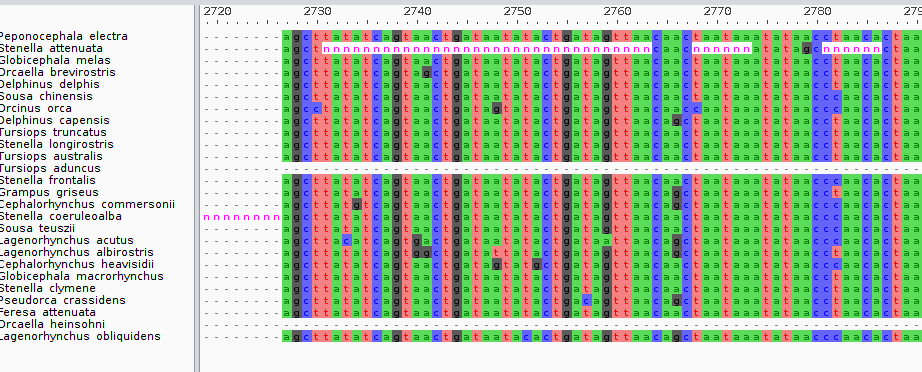
\includegraphics[scale = 0.5, angle = 90]{alignfasta.png}
    \caption{Aligned Fasta in aliview}
    \label{fig:aliview}
\end{figure} 
\newpage
\begin{figure}
    \centering
    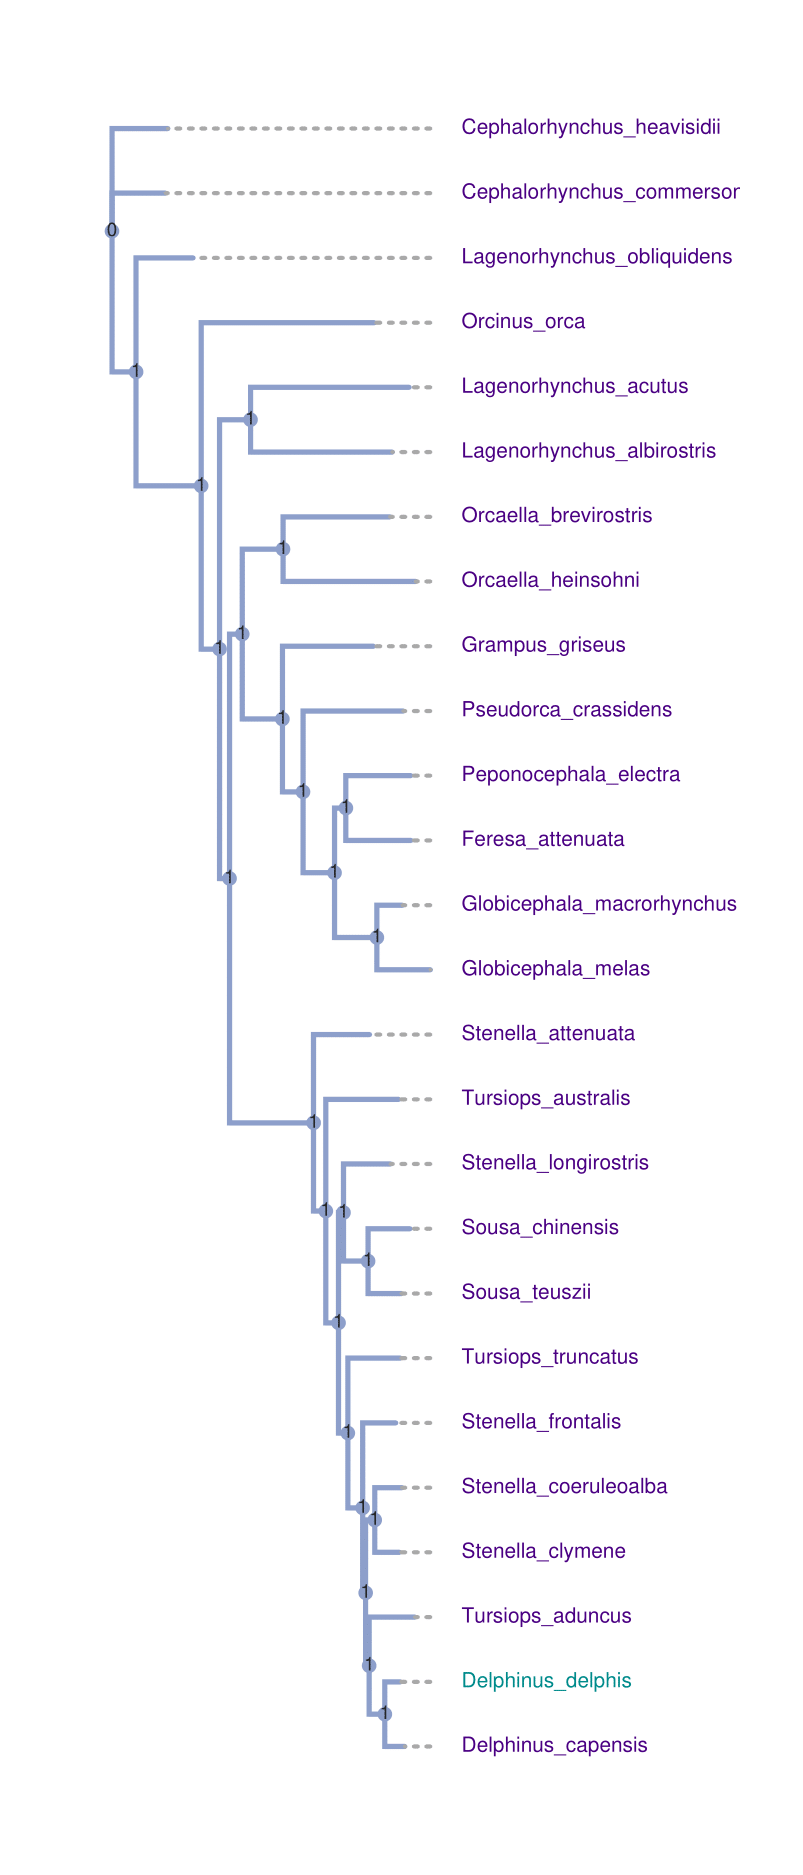
\includegraphics[scale = 0.9]{tree-plot_MB-1.png}
    \caption{Phylogenetic Tree of the Program}
    \label{fig:ourPhy}
\end{figure}
\newpage
\begin{figure}
    \centering
    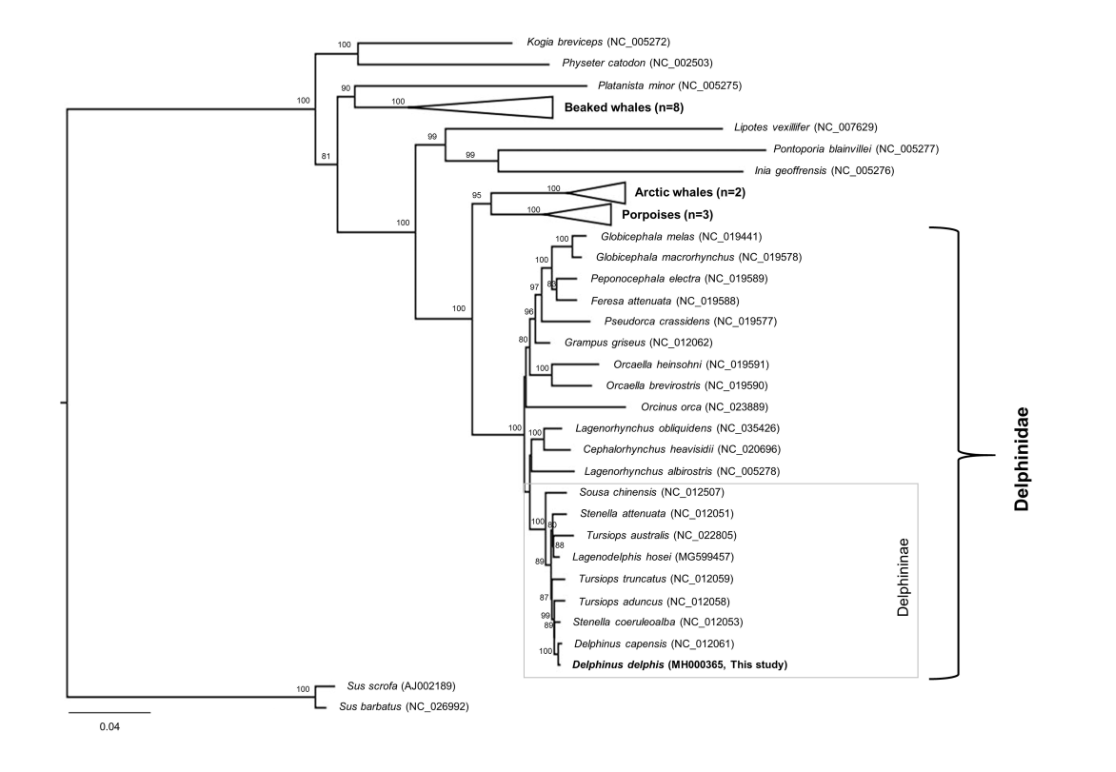
\includegraphics[scale = 0.55]{Delphinus_tree_1.png}
    \caption{Phylogenetic Tree of the article}
    \label{fig:theirPhy}
\end{figure}

\end{document}


